\documentclass[usenames,dvipsnames]{beamer}

% Cargar el tema
\usetheme{metropolis}

% Configuración de LaTeX
\usepackage[spanish]{babel}
\usepackage[utf8]{inputenc}

\usepackage{listings}


\usepackage{graphicx,wrapfig,lipsum}

% Configuración básica del tema
\metroset{
  % tema oscuro ('dark') o claro ('light'). No tiene efecto al usar la
  % paleta de colores más adelante
  background=light,
  % 'none' para eliminar la diapositiva inicial de cada sección
  sectionpage=progressbar,
  % 'progressbar' o 'simple' para añadir una diapositiva inicial a cada subsección
  subsectionpage=none,
  % contador de página: 'none', 'counter' o 'fraction'
  numbering=none,
  % barra de progreso: 'none', 'head', 'frametitle' o 'foot'
  progressbar=frametitle,
  % fondo de los bloques estilo teorema: 'transparent' o 'fill'
  block=fill,
}


% Paleta de colores
\definecolor{accent}{RGB}{151, 186, 88}
\colorlet{darkaccent}{accent!70!black}
\definecolor{foreground}{RGB}{0, 0, 0}
\definecolor{background}{RGB}{255, 255, 255}

% Insertar los colores en el tema
\setbeamercolor{normal text}{fg=foreground, bg=background}
\setbeamercolor{alerted text}{fg=darkaccent, bg=background}
\setbeamercolor{example text}{fg=foreground, bg=background}
\setbeamercolor{frametitle}{fg=background, bg=accent}

\setbeamercolor{headtitle}{fg=background!70!accent,bg=accent!90!foreground}
\setbeamercolor{headnav}{fg=background,bg=accent!90!foreground}
\setbeamercolor{section in head/foot}{fg=background,bg=accent}

%
\defbeamertemplate*{headline}{miniframes theme no subsection}{
  % Caja para mostrar título y autor encima de cada diapositiva
  % Nosotros no 
  %% \begin{beamercolorbox}[ht=2.5ex,dp=1.125ex,
  %%     leftskip=.3cm,rightskip=.3cm plus1fil]{headtitle}
  %%   {\usebeamerfont{title in head/foot}\insertshorttitle}
  %%   \hfill
  %%   \leavevmode{\usebeamerfont{author in head/foot}\insertshortauthor}
  %% \end{beamercolorbox}
  %% \begin{beamercolorbox}[colsep=1.5pt]{upper separation line head}
  %% \end{beamercolorbox}

  % Caja para mostrar navegación encima de cada diapositiva
  \begin{beamercolorbox}{headnav}
    \vskip2pt\insertnavigation{\paperwidth}\vskip2pt
  \end{beamercolorbox}
  \begin{beamercolorbox}[colsep=1.5pt]{lower separation line head}
  \end{beamercolorbox}
}

%eye-candy; sintasix más bonita
\newcommand{\seccion}[1]{\input{./sections/#1}}
\newcommand{\foo}{\hspace{-2.3pt}$\bullet$ \hspace{5pt}}

%Meta


\subtitle{Un método iterativo y creciente}
\title{DSDM: Dynamic System Development
Method}
\date{}
\institute{Universidad de Granada}
\author{Pedro Bonilla Nadal\\
David Infante Casas\\
Laura Gómez Garrido\\
Antonio Martín Ruiz\\
Juan Ocaña Valenzuela}
%\titlegraphic{\hfill\includegraphics[height=1.5cm]{./logo_mifare.png}}


\begin{document}
\maketitle
\begin{frame}{Contenidos.}
  \setbeamertemplate{section in toc}[sections numbered]
  \tableofcontents [hideallsubsections]
\end{frame}

\section{Introducción}
\begin{frame}{Introducción}
El método de desarrollo de sistemas dinámicos (Dynamic Systems Development Method, DSDM) es un framework para el desarrollo de software de forma ágil. Esta metodología determina fases, subfases y principios que permiten a equipos de desarrollo trabajar de forma eficiente.

\end{frame}

\begin{frame}{Introducción}
    \centering
        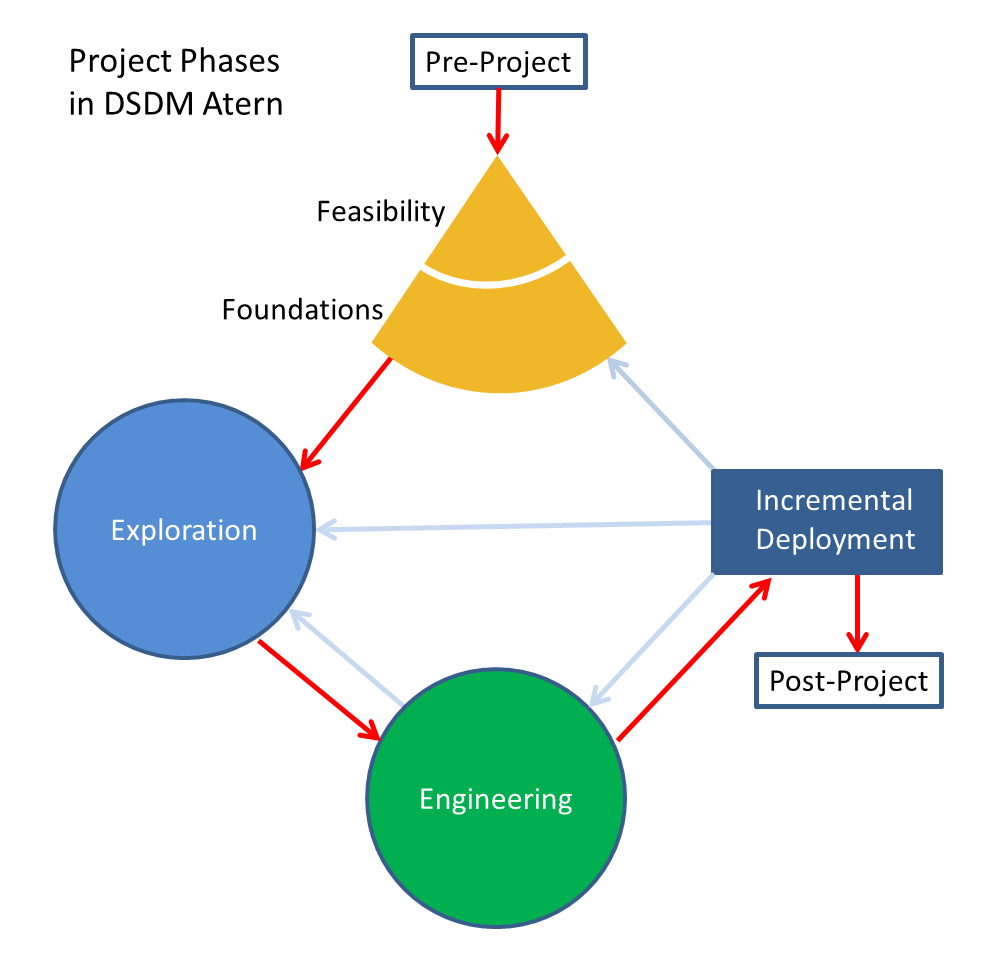
\includegraphics[width=0.7\textwidth]{DSDM_Phases.png}
\end{frame}



\section{Roles}
\begin{frame}{Roles}
    \begin{itemize}
        \item Patrocinador ejecutivo
        \item Visionario
        \item Usuario embajador
        \item Project Manager
        \item Desarrolladores
        \item Testers
    \end{itemize}{}
\end{frame}{}


\section{Fases de desarrollo}
\begin{frame}{Fases}
    \begin{itemize}
        \item Pre-proyecto. 
\item Ciclo de vida del proyecto. Está formado por las siguientes fases:
\begin{itemize}
    \item Viabilidad
    \item Fundaciones
    \item Exploración
    \item Ingeniería
    \item Despliegue
\end{itemize}{}
\item Post proyecto.

    \end{itemize}{}
\end{frame}


\section{Principios}

\begin{frame}{Principios}
    \begin{enumerate}
        \item Participacion activa del usuario.
        \item Los equipos deben poder tomar decisiones.
        \item Concentrarse en los límites de entrega.
        \item Considerar como criterio la validez en el mercado del producto.
        \item Desarrollo iterativo e incremental.
        \item Todos los cambios durante el desarrollo deben ser reversibles.
        \item Los requisitos se definen a alto nivel.
        \item Las pruebas están integradas de manera continua.
        \item Enfoque colaborativo y cooperativo.
    \end{enumerate}{}
\end{frame}{}

\section{Valores}

\begin{frame}{Valores}
    \begin{itemize}
        \item Individuos
        \item Software funcional
        \item Colaboración
        \item Respuesta al cambio
    \end{itemize}
\end{frame}{}



\section{TimeBoxing}

\begin{frame}{Timebox}
    TimeBoxing es una técnica muy útil para lograr el mismo resultado. Una TimeBox es un intervalo, normalmente no más largo de 6 semanas, donde un conjunto da do de tareas debe ser logrado.
\end{frame}{}


\begin{frame}[standout]
  ¡Muchas gracias!
\end{frame}
\end{document}
